\documentclass[a4paper,12pt]{article}

\usepackage[utf8]{inputenc}
\usepackage[T1]{fontenc}
\usepackage{graphicx}
\usepackage{float}
\usepackage{geometry}
\usepackage{booktabs}
\usepackage{tikz}

\usetikzlibrary{arrows.meta,positioning}

\geometry{margin=2.5cm}

\setlength{\parindent}{0pt}
\setlength{\parskip}{0.5em}

\title{Bericht}
\author{Jiaqi Wang}
\date{\today}

\begin{document}

\maketitle

\section{Einführung}

In dieser Woche wurde die Ansteuerung eines Schrittmotors mit einem ESP32-S3 umgesetzt. Dabei wurden sowohl eine Open-Loop-Steuerung als auch eine Closed-Loop-Steuerung mithilfe eines Drehgebers realisiert. Zusätzlich wurde eine TCP-Kommunikation über WLAN implementiert, um den Motor drahtlos steuern zu können.

\begin{figure}[H]
    \centering
    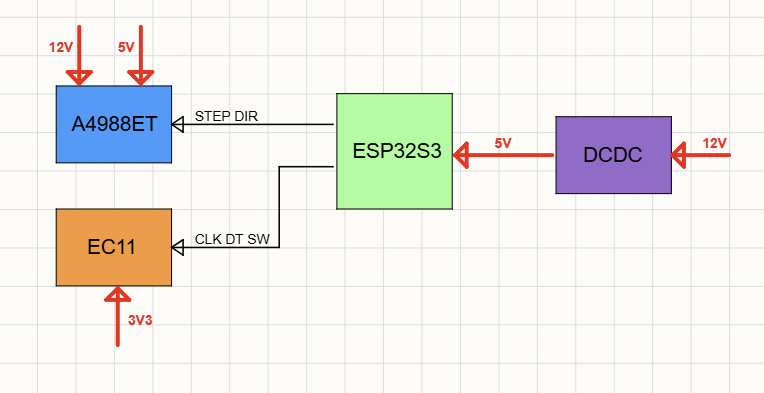
\includegraphics[width=0.85\textwidth]{overview.png}
    \caption{Systemübersicht des Versuchsaufbaus}
    \label{fig:overview}
\end{figure}

\section{Schrittmotor und Motortreiber}

Für den Versuchsaufbau wurde ein Schrittmotor des Typs \textbf{17HM5417} mit einem Schrittwinkel von \textbf{1,8°} verwendet. Die Ansteuerung erfolgte über den Motortreiber \textbf{A4988}.

Im Vollschrittbetrieb beträgt die theoretische Schrittzahl für eine vollständige Umdrehung:

\[
\frac{360^\circ}{1.8^\circ}=200
\]

Somit sollte der Motor nach 200 Schritten genau eine Umdrehung ausführen.


Die Ansteuerung des Schrittmotors erfolgt über die STEP- und DIR-Signale des A4988-Treibers.
Das folgende Programmfragment zeigt die grundlegende Motorsteuerung.

\begin{verbatim}
void stepMotor(int steps, bool dir) {
  digitalWrite(DIR_PIN, dir);

  for (int i = 0; i < steps; i++) {
    digitalWrite(STEP_PIN, HIGH);
    delayMicroseconds(1000);
    digitalWrite(STEP_PIN, LOW);
    delayMicroseconds(1000);
  }
}
\end{verbatim}


Während der ersten Tests wurde eine Open-Loop-Steuerung implementiert. Obwohl theoretisch 200 Schritte einer vollständigen Umdrehung entsprechen, rotierte der Motor nur etwa $10^\circ$ bis $20^\circ$. Eine mögliche Ursache ist die hohe mechanische Reibung der Lagerung. Daher wurde anschließend eine Closed-Loop-Steuerung mit Drehgeber entwickelt.

\begin{figure}[H]
\centering

\begin{tikzpicture}[>=Stealth]

\node[draw, minimum width=2.5cm, minimum height=1.5cm] (H) {H};

\draw[->] (-2,0) -- (H.west) node[midway, above] {$x$};
\draw[->] (H.east) -- +(2,0) node[midway, above] {$y$};

\end{tikzpicture}

\caption{Blockdiagramm einer Open-Loop-Steuerung}
\end{figure}

Dabei beschreibt (x) den Sollwinkel und (y) die resultierende Position des Motors. Das Übertragungsglied (H) umfasst den ESP32-S3, den Motortreiber A4988 sowie den Schrittmotor.



Zur Verbesserung der Positioniergenauigkeit wurde ein EC11-Drehgeber in das System integriert. Der Drehgeber ist mechanisch mit der Motorwelle gekoppelt und liefert kontinuierlich Positionsinformationen an den ESP32-S3.

\begin{verbatim}
void IRAM_ATTR encoderISR() {
  int clkValue = digitalRead(ENCODE_CLK);
  int dtValue = digitalRead(ENCODE_DT);

  if (lastCLK != clkValue) {
    lastCLK = clkValue;

    if (clkValue != dtValue) {
      encoderCount++;
    } else {
      encoderCount--;
    }
  }
}
\end{verbatim}

Die Signale CLK und DT des Encoders werden über Interrupts ausgewertet. Aus den erfassten Impulsen berechnet der ESP32 die aktuelle Winkelposition der Motorwelle. Anschließend wird diese Position mit dem vorgegebenen Sollwinkel verglichen.

Bei Abweichungen zwischen Soll- und Istwert erzeugt der ESP32 zusätzliche STEP-Signale für den A4988-Treiber, bis die gewünschte Position erreicht ist. Dadurch entsteht ein Closed-Loop-Regelkreis, der Positionsfehler automatisch korrigieren kann.


\begin{figure}[H]
\centering

\begin{tikzpicture}[>=Stealth]

% Summierstelle
\node[circle, draw, minimum size=8mm] (sum) at (0,0) {$+$};

% Systemblock
\node[draw, minimum width=2.5cm, minimum height=1.5cm] (H) at (4,0) {H};

% Eingang
\draw[->] (-2,0) -- (sum) node[midway, above] {$x$};

% Ausgang
\draw[->] (sum) -- (H.west);
\draw[->] (H.east) -- +(2,0) node[midway, above] {$y$};

% Rückführung
\draw[-] (6,0) -- (6,-2);
\draw[-] (6,-2) -- (0,-2);
\draw[->] (0,-2) -- (sum.south);

% Minuszeichen
\node at (-0.5,-0.5) {$-$};

\end{tikzpicture}

\caption{Blockdiagramm einer Closed-Loop-Steuerung}
\end{figure}


Im Gegensatz zur Open-Loop-Steuerung ermöglicht dieses Verfahren eine höhere Genauigkeit. Die aktuelle Positionsabweichung zwischen Sollwinkel und Istwinkel beträgt jedoch noch etwa \(10^\circ\).


\section{TCP-Kommunikation über WLAN}

Neben der Motorsteuerung wurde eine TCP-basierte Kommunikation über WLAN implementiert. Der ESP32-S3 fungiert dabei als TCP-Server und wartet auf eingehende Verbindungen eines Clients.

Nach dem Verbindungsaufbau können Steuerbefehle über das Netzwerk an den ESP32-S3 gesendet werden. Die empfangenen Daten werden verarbeitet und anschließend zur Ansteuerung verschiedener Funktionen des Systems verwendet.



Zusätzlich wurde mit dem Qt-Framework eine einfache grafische Benutzeroberfläche entwickelt. Die Anwendung dient als TCP-Client und ermöglicht die drahtlose Kommunikation mit dem ESP32-S3.

\begin{figure}[H]
\centering
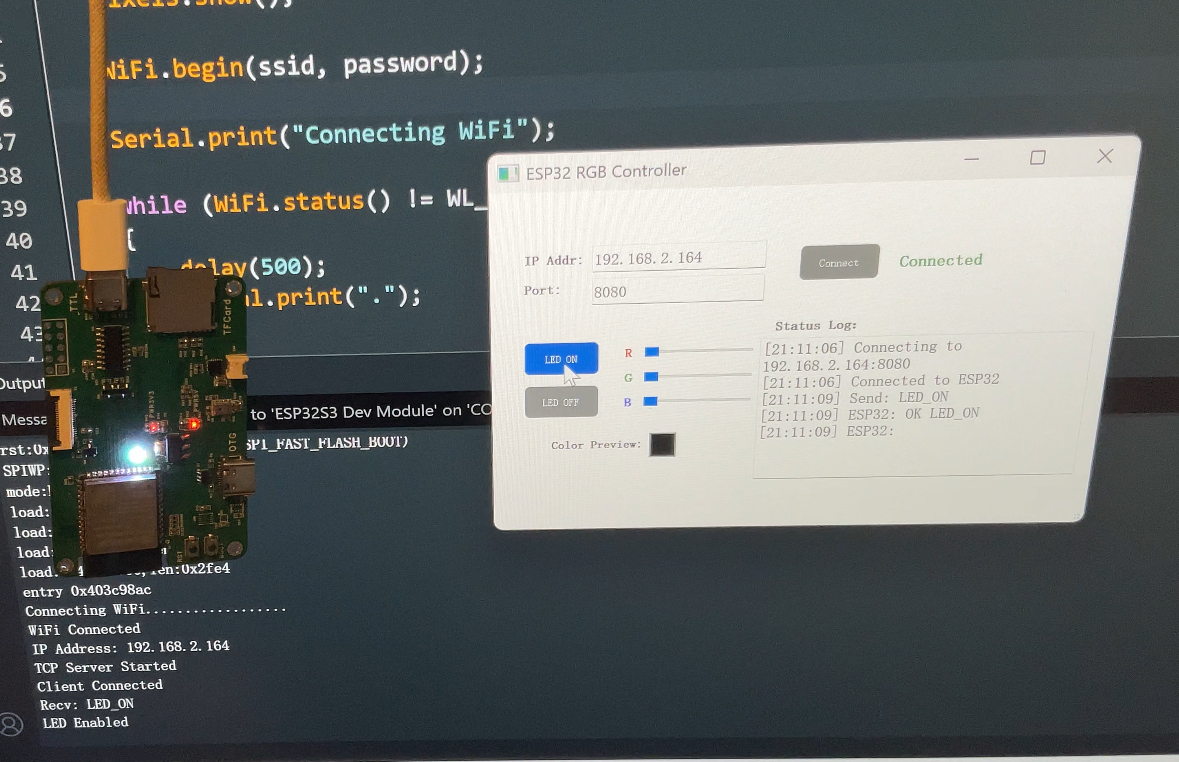
\includegraphics[width=0.6\textwidth]{hostpc.jpg}
\caption{Qt-basierte Benutzeroberfläche zur Kommunikation mit dem ESP32-S3}
\end{figure}

Über die Benutzeroberfläche können Befehle an den Mikrocontroller gesendet werden. Im Rahmen eines ersten Tests wurde die auf dem ESP32-S3 integrierte WS2812-RGB-LED erfolgreich drahtlos angesteuert. Dadurch konnte die TCP-Kommunikation zwischen PC und Mikrocontroller erfolgreich verifiziert werden.



\end{document}
